\documentclass{ituthesis}
\usepackage[]{hyperref}
\usepackage[]{float} 
\usepackage[]{csquotes} 
\usepackage[]{graphicx} 
\usepackage[]{caption} 
\usepackage[]{subcaption} 
\usepackage[]{natbib}
\usepackage[]{mdframed}
\usepackage[]{amsthm} 
\bibliographystyle{agsm}

\definecolor{constructor-color}{RGB}{155,187,89}
\definecolor{type-color}{RGB}{142,180,227}
\definecolor{declared-var-color}{RGB}{192,80,77}
\definecolor{local-var-color}{RGB}{230,185,184}
\definecolor{literal-color}{RGB}{179,162,199}

\newcommand{\ttconstructor}[1]{\textcolor{constructor-color}{\texttt{#1}}}
\newcommand{\tttype}[1]{\textcolor{type-color}{\texttt{#1}}}
\newcommand{\ttdec}[1]{\textcolor{declared-var-color}{\texttt{#1}}}
\newcommand{\ttvar}[1]{\textcolor{local-var-color}{\texttt{#1}}}
\newcommand{\ttliteral}[1]{\textcolor{literal-color}{\texttt{#1}}}

\theoremstyle{definition}
\newtheorem{exmp}{Example}

\newenvironment{asideblock}
  {\begin{mdframed}[style=0,%
      leftline=false,rightline=false,leftmargin=2em,rightmargin=2em,%
          innerleftmargin=0pt,innerrightmargin=0pt,linewidth=0.75pt,%
      skipabove=7pt,skipbelow=7pt]\small}
  {\end{mdframed}}

\settitle{The Practical Guide to Levitation}
\setauthor{Ahmad Salim Al-Sibahi}
\setsupervisor{Dr. Peter Sestoft}
\setextrasupervisor{David R. Christiansen}
\setdate{September 1, 2014}

\begin{document}
%\selectlanguage{danish}

\frontmatter

\thetitlepage
\newpage

\chapter*{Abstract}
Goal: Implementation of levitation in a realistic setting, with practical performance benefits.
\blockquote{DISCLAIMER: This is a draft and as such is incomplete, incorrect and can contain grammatical errors.
Although I claim originality of this report, many underlying ideas are based on current work in the scientific community which will be correctly attributed
when the work is complete.}

\cleardoublepage
\setcounter{tocdepth}{1}
\tableofcontents

\mainmatter

%from memoir documentation:
%TeX tries very hard to keep text lines justified while keeping the interword spacing as constant as possible, but sometimes fails and complains about an overfull hbox.
%The default mode for LaTeX typesetting is \fussy where the (variation of) interword spacing in justified text is kept to a minimum. Following the \sloppy declaration there may be a much looser setting of justified text.
%Additionally the class provides the \midsloppy declaration which allows a setting somewhere between \fussy and \sloppy.
%fewer overfull lines than \fussy, and fewer obvious large interword spacing than with \sloppy.
%the memoir manual also uses \midsloppy!
\midsloppy
% try harder to avoid widows and orphans
\sloppybottom

\chapter{Introduction}
\label{cha:Intoduction}
\section{Context}
\label{sec:Context}
Algebraic datatypes such as Boolean values, lists or trees form a core part of modern functional programming.
Most functions written work directly on such datatypes, but sometimes it is the case that there are functions that don't directly dependent on the datatype itself and only are there to serve as a repetitive exercise; For example, in cases as structural equality or pretty printing (see Example~\ref{exmp:prettyprint}).
In fact it is possible to write an algorithm over the structural definition of the datatype, which the computer then could use to derive an actual function for particular datatypes.

\begin{exmp}
  Pretty printing a data for any algebraic data type follows a very simple step of procedures:
  \begin{enumerate}
    \item Print the name of the constructor
    \item Iterate through the data elements and pretty print them, with all the data surrounded by parentheses if necessary
    \begin{enumerate}
      \item If the data element is a recursive reference to the type itself, then call this procedure recursively (starting at point 1.)
      \item If the data element is of another type
      \begin{enumerate}
        \item Find the correct pretty printing function for that type
        \item Pretty print the field using the found function
      \end{enumerate}
    \end{enumerate}
    \item Finish printing
  \end{enumerate}
  \label{exmp:prettyprint}
\end{exmp}

Enter the world of \textit{generic programming} where the target datatype is the one describing the structure of other datatypes, often called the \textit{description}.
While generic programming sounds promising, it is usually seen as a challenging aspect of Haskell\,\cite[]{haskell98} to use by ordinary programmers. To represent the description, it is often required to use special language extensions\,\cite[]{magalhaes2010generic} and the programming style tends to require different abstractions than when writing ordinary programs.

%A tiny bit of history here?
However, in dependently-typed languages such as Idris\,\cite[]{brady2013idris} or Agda\,\cite[]{norell2009dependently} that it is possible to mitigate such issues.
Due to the nature of dependently-typed languages it is possible to create a correct description using ordinary datatype definitions\,\cite[]{benke2003universes}.
Furthermore, \cite{Chapman:2010:GAL:1863543.1863547} show that it is possible to build a self-supporting closed type system which is able to convert these descriptions to ordinary types (creating so-called \textit{described types}), while still being powerful enough to describe the description datatype itself.
Therefore in such system, generic programming is just a special case of ordinary programming.

%\subsection{The Importance of Genericity in Dependently-typed Languages}
%\label{sub:TheImportanceofGenericityinDependently-typedLanguages}
%\textit{The similarity of structure and various slightly-different indexing of types.}


\section{Problem definition}
\label{sec:ProblemDefinition}
The current work on generic programming in dependently-typed languages presents both elegant and typesafe ways to represent the structural descriptions of datatypes.
Furthermore, it allows the programmer to save both time and boilerplate code while reducing mistakes by using ordinary programming techniques to do generic programming.

However, the state of the art is heavily theoretically oriented, which might lead to issues when a system needs to be developed with a practical audience in mind.
First of all, multiple description formats are often presented, sometimes even in the same paper, which might not be particularly attractive in a practical setting.
Secondly, there has been little work done on how to integrate such descriptions in languages which contain features such as type classes and proof scripts.
Finally, datatypes synthesised from descriptions create large canonical terms thus, both type checking and runtime performance are very slow.
In summary, if an efficient and easily usable framework for programming with described types that avoids the described issues could be implemented successfully, it would save programmers both the time and effort required to write repetitive functions.

\section{Aim and scope}
\label{sec:AimandScope}
The aim of this research is to provide a practical and efficient implementation of described types in Idris.
This project has three primary subgoals.

The first subgoal is to find a good definition of the description that supports many common datatypes.
I seek to mainly reuse some of the existing work, and not try to improve underlying type theory to support more complex inductive families; neither will I focus on supporting all language features of Idris such as implicit arguments and codata definitions.

The second subgoal is to present realistic examples using generic functions working on described types. 
This mainly includes implementing functions that can be used to derive type class instances, and a Scrap Your Boilerplate (SYB) library for generic querying and traversal.

The final subgoal is that I seek to use partial evaluation to optimise the generic functions with regards to specific descriptions in order to achieve acceptable performance.
This includes using techniques such as polyvariant partial evaluation and constructor specialisation. %Elaborate when I know more about PE\ldots

\section{Significance}
\label{sec:Significance}
The main contributions of this thesis are:

\begin{itemize}
  \item an example-based tutorial for understanding described types in the context of a practical programming language, namely Idris
  \item an generic implementation of common operations such as decidable equality, pretty printing and functors, which can be used to provide default implementations to type class methods.
  \item a discussion of the challenges that arise when trying to implement a SYB-style generics library in dependently typed languages
  \item optimisation techniques based on partial evaluation for reducing runtime size and time overhead for described types and accompanying generic functions
  \item metrics showing that generic programming using described types is a viable option to reduce boilerplate without significant cost in performance
\end{itemize}
\section{Overview}
\label{sec:Overview}

The report is structured as follows. Chapter~\ref{cha:GenericProgramming}, presents an introduction to described types specifically focusing on recent developments using dependently-typed programming languages.
Chapter~\ref{cha:PartialEvaluation}, presents an overview of techniques for partial evaluation of functions and specialisation of datatypes. Chapter~\ref{cha:LevitatingIdris}, discusses specifically how described types are implemented in Idris and continues with practical examples in Chapter~\ref{cha:PracticalExamples}.
Chapter~\ref{cha:OptimizingIdrisforFlight} presents what optimisations were made in order to improve the runtime performance of described types and generic functions. Evaluation of the results happens in Chapter~\ref{cha:Evaluation}, comparing the performance of generic implementations to hand-written ones.
Finally, Chapter~\ref{cha:Discussion} discusses what challenges still lie ahead and concludes the effort.
\chapter{Generic programming}
\label{cha:GenericProgramming}
\section{The generic structure of inductive data types}
\label{sec:TheGenericStructureofInductiveDataTypes}
\subsection{Anatomy of a datatype}
\label{sub:AnatomyofaDatatype}
To build an intuition that will be useful in understanding descriptions, let us first start by looking closely at how datatypes are structured.
Figure~\ref{fig:anatomydatatype}, presents an annotated version of a typical dependently-typed datatype representing vectors.

\begin{figure}[ht]
\begin{center}
    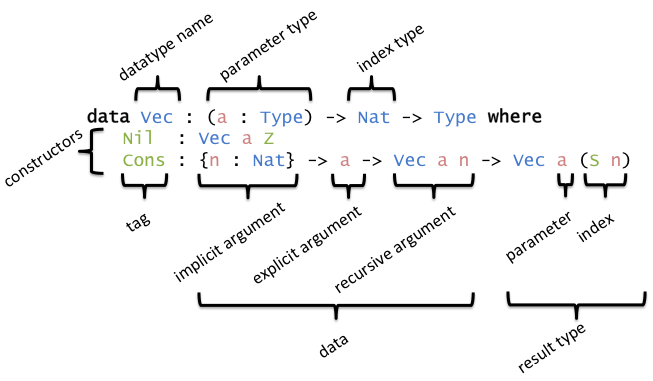
\includegraphics[scale=0.5]{Figures/AnatomyOfADatatype.png}
\end{center}
\caption{Annotated components of a datatype Declaration}
\label{fig:anatomydatatype}
\end{figure}

A datatype consists of a type constructor which describes what type-level arguments are required, and zero or more data constructors which describe how to create values of the datatype.
The type constructor has three components: a name for the datatype, types of any possible parameters, and the types of possible indices.
In Figure~\ref{fig:anatomydatatype} there is no syntactic difference between a parameter type or an index type since Idris figures that out automatically.\footnote{If an argument to a type constructor doesn't change in the data constructor declarations, Idris considers it a parameter, otherwise an index.}

Similarly to the type constructor, a data constructor needs a name, also called a \textit{tag}.
Following the tag, the data constructor declaration contains the types of the arguments stored in the constructor and the resulting type which must use the type constructor of the datatype.
In our example two constructors are declared, \ttconstructor{Nil} and \ttconstructor{Cons}.
Constructor \ttconstructor{Nil} doesn't hold any data, so it only needs to define the resulting type which is \tttype{Vec}~\ttvar{a}~\ttconstructor{Z} (a vector with length \ttliteral{0}).
Constructor \ttconstructor{Cons} contains three different types of arguments: an ordinary implicit argument, an ordinary explicit argument, and an explicit argument of the type itself (recursive); the resulting type for \ttconstructor{Cons} is \tttype{Vec}~\ttvar{a}~\texttt{(}\ttconstructor{S}~\ttvar{n}\texttt{)}, that is, a vector of length \ttliteral{1}\texttt{+}\ttvar{n} where \ttvar{n} is the length of the recursive argument.

\begin{asideblock}
  The colouring scheme for code presented in this paper uses the following conventions:
  \begin{quote}
  \begin{description}
    \item[\tttype{Blue}] is used for type constructors
    \item[\ttconstructor{Green}] is used for data constructors
    \item[\ttdec{Dark Red}] is used for top-level declarations
    \item[\ttvar{Light Red}] is used for locally-bound variables
    \item[\ttliteral{Purple}] is used for literals (integer, string, etc.)
  \end{description}
  \end{quote}

\end{asideblock}

\subsection{A description for datatypes}
\label{sub:ADescriptionforDatatypes}
It is now possible to try to represent a suitable description datatype. Figure~\ref{fig:descriptiondatatype} presents one possible solution, influenced mainly by the work of \cite{mcbride2010ornamental} and \cite{diehl2014eliminators}.

\begin{figure}[ht]
\begin{center}
    \includegraphics[scale=0.5]{Figures/ADescriptionforDatatypesSimple.png}
\end{center}
\caption{A datatype that describes other datatypes}
\label{fig:simpldescdatatype}
\end{figure}

The description datatype has three main constructors:
\begin{itemize}
  \item  Constructor \ttconstructor{Ret} represents the end of a description
  \item  Constructor \ttconstructor{Arg} represents the addition of an argument of any type to a given description; the first argument of \ttconstructor{Arg} is the type of argument expected and the second argument is the rest of the description dependent on a value of that type.
  \item  Constructor \ttconstructor{Rec} represents an recursive argument of the described datatype. The argument of constructor \ttconstructor{Rec} is the specification of the rest of the description.
\end{itemize}

In order to get an idea on how descriptions for various interesting datatypes look like, the following paragraphs will show a series of examples providing a side-by-side comparison of ordinary declarations to descriptions.
The declaration of the trivial singleton type \tttype{Unit} is shown in Figure~\ref{fig:declunit}, and its corresponding description is shown in Figure~\ref{fig:descunit}.
Since the sole constructor \ttconstructor{MkUnit} doesn't contain any arguments, \ttconstructor{Ret} is used to simply end the description.

\begin{figure}[ht]
\begin{center}
  \subcaptionbox{Declaration of \tttype{Unit}\label{fig:declunit}}[.45\textwidth]{
    
\includegraphics[scale=0.5]{Figures/UnitDeclaration.png}
}
\subcaptionbox{Description of \tttype{Unit}\label{fig:descunit}}[.45\textwidth]{
    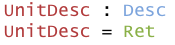
\includegraphics[scale=0.5]{Figures/UnitDescription.png}

}
\caption{The \tttype{Unit} datatype and its description}
\end{center}
\end{figure}

A more interesting datatype is shown in Figure~\ref{fig:declpair}, namely the datatype \tttype{Pair} representing a pair of \tttype{Int} and \tttype{Bool}.
The translation to the corresponding description, as shown in Figure~\ref{fig:descpair}, seems straightforward. For each argument of \ttconstructor{MkPair}, we use
would be of the form \ttconstructor{Arg}~\ttvar{a}~\texttt{(\textbackslash}\ttvar{arg}~\texttt{=>}~\ttvar{b}\texttt{)}
Finally, to specify the end of the description, \ttconstructor{Ret} is used.

\begin{figure}[ht]
\begin{center}
  \subcaptionbox{Declaration of \tttype{Pair}\label{fig:declpair}}[.45\textwidth]{
    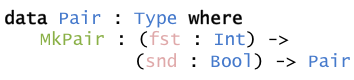
\includegraphics[scale=0.5]{Figures/PairDeclaration.png}
}
\subcaptionbox{Description of \tttype{Pair}\label{fig:descpair}}[.45\textwidth]{
    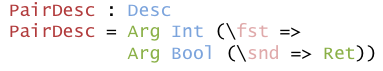
\includegraphics[scale=0.5]{Figures/PairDescription.png}

}
\caption{A pair of \tttype{Int} and \tttype{Bool}}
\end{center}
\end{figure}

A key aspect of algebraic datatypes is the ability to choose between multiple constructors.
Figure~\ref{fig:decleither} shows a simple datatype \tttype{Either} which provides two constructors \ttconstructor{Right} and \ttconstructor{Left}, than can hold a value of \tttype{Int} and \tttype{String} respectively.

Since there is no explicit way to encode a choice between multiple constructor in the provided description, instead, a boolean argument \ttvar{isRight} is used to determine which constructor is described.
If the value of \ttvar{isRight} is true then the resulting description is expected to be for the \ttconstructor{Right} constructor, otherwise
is is expected to be for the \ttconstructor{Left} constructor. The description for each constructor is then specified in a similar fashion to datatypes with one constructor such
as \tttype{Pair} described above.

\begin{figure}[ht]
\begin{center}
  \subcaptionbox{Declaration of \tttype{Either}\label{fig:decleither}}[.45\textwidth]{
    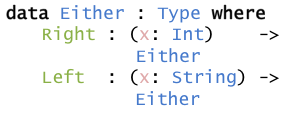
\includegraphics[scale=0.5]{Figures/EitherDeclaration.png}
}
\subcaptionbox{Description of \tttype{Either}\label{fig:desceither}}[.45\textwidth]{
    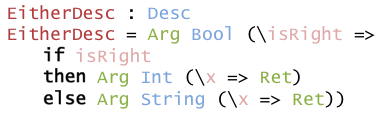
\includegraphics[scale=0.5]{Figures/EitherDescription.png}

}
\caption{the sum type of \tttype{Int} and \tttype{String}}
\end{center}
\end{figure}

In addition to allowing the choice between multiple possible constructors, what makes algebraic datatypes interesting is the ability to
have recursive (or \textit{inductive}) instances. The simplest recursive datatype is the natural numbers \tttype{Nat} (shown in Figure~\ref{fig:declnat}) which has two constructors,
\ttconstructor{Zero} which represents \ttliteral{0} and the recursively defined \ttconstructor{Succ} which represents \ttliteral{1}+\ttvar{n} for any natural number \ttvar{n}.
The corresponding description is shown in Figure~\ref{fig:declnat} which is mainly built up using the principles introduced before.
The only addition is that the description for \ttconstructor{Succ} now uses \ttconstructor{Rec} to specify that it requires a recursive argument (to type \tttype{Nat} itself).

\begin{figure}[ht]
\begin{center}
  \subcaptionbox{Declaration of \tttype{Nat}\label{fig:declnat}}[.45\textwidth]{
    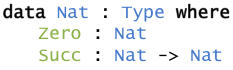
\includegraphics[scale=0.5]{Figures/NatDeclaration.png}
}
\subcaptionbox{Description of \tttype{Nat}\label{fig:descnat}}[.45\textwidth]{
    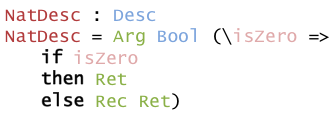
\includegraphics[scale=0.5]{Figures/NatDescription.png}

}
\caption{The Natural numbers (\tttype{Nat})}
\end{center}
\end{figure}

Figure~\ref{fig:decllist} shows one of the classical datatypes in functional programming languages, namely \tttype{List}.
Unlike \tttype{Pair} and \tttype{Either} which were monomorphic in the presented examples, this time \tttype{List} is polymorphic in its elements.
The way to represent parameters is by having them as arguments to the function describing the particular datatype, which allows them to be qualified over the whole description.
The description itself is built using the previously described methods and is shown in Figure~\ref{fig:desclist}. There is a Boolean argument \ttvar{isNil}, which encodes the choice between the two constructors of the list,
\ttconstructor{Nil} and \ttconstructor{Cons}. The description for \ttconstructor{Nil} is simply \ttconstructor{Ret} since it doesn't accept any arguments, and the description for \ttconstructor{Cons} takes an argument of the parameter type (the head of the list)
a recursive argument (the tail of the list) and ends the description.

\begin{figure}[ht]
\begin{center}
  \subcaptionbox{Declaration of \tttype{List}\label{fig:decllist}}[.45\textwidth]{
    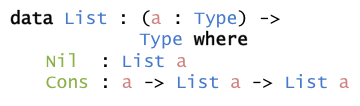
\includegraphics[scale=0.5]{Figures/ListDeclaration.png}
}
\subcaptionbox{Description of \tttype{List}\label{fig:desclist}}[.45\textwidth]{
    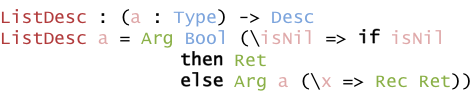
\includegraphics[scale=0.5]{Figures/ListDescription.png}

}
\caption{A polymorphic list of elements}
\end{center}
\end{figure}

\subsection{Indexing descriptions}
\label{sub:Indexingdescriptions}

In order to allow datatypes to be indexed by values, the description structure takes a parameter that describes what the type of indices must be.
Figure~\ref{fig:descriptiondatatype} shows an updated version of Figure~\ref{fig:simpldescdatatype}, that contains the necessary parameter \ttvar{ix} for indexing datatypes.
The constructors \ttconstructor{Ret} and \ttconstructor{Rec}, must also be updated to take a value of \ttvar{ix} in order to represent what the index of the result type and recursive argument must be respectively.
For descriptions that don't require indices, they can be converted to indexed descriptions using the unit type \tttype{Unit} (or using its syntactic form \tttype{()}) as index.

\begin{figure}[ht]
\begin{center}
    \includegraphics[scale=0.5]{Figures/ADescriptionforDatatypes.png}
\end{center}
\caption{Description for datatypes with possible indices}
\label{fig:descriptiondatatype}
\end{figure}

In order to given an example on how an indexed datatype looks like, let us take a new look at \tttype{Vec} from Figure~\ref{fig:anatomydatatype}.
Figure~\ref{fig:descvec} shows the corresponding description of \tttype{Vec} with comparable annotations.

\begin{figure}[ht]
\begin{center}
    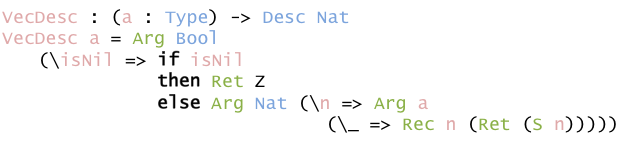
\includegraphics[scale=0.5]{Figures/VectorDescription.png}
\end{center}
\caption{Described version of \tttype{Vec}}
\label{fig:descvec}
\end{figure}


The type signature for the description of \tttype{Vec} mimics the one for the actual datatype closely, but there are nonetheless some differences.
There is now an explicit distinction between parameters and indices; the type for a parameter can still be specified as an argument for the description value,
whereas the type of an index must be provided to the \tttype{Desc} type constructor.
This is to ensure that all provided indices conform to same expected type, while still allowing the values to change inside the description.

A Boolean argument \ttvar{isNil} is used to describe the choice between constructors \ttconstructor{Nil} and \ttconstructor{Cons}.
The constructor \ttconstructor{Nil} doesn't contain any data so we simply use \ttconstructor{Ret~Z}, which indicates that the description is finished and the resulting type is expected to have index \ttconstructor{Z}, analogously to Figure~\ref{fig:anatomydatatype}.
The constructor \ttconstructor{Cons} takes first two ordinary arguments: a \tttype{Nat} argument
to be used to describe the necessary indices, and an argument of the parameter \ttvar{a}. Following these arguments we take a recursive argument---specified using \ttconstructor{Rec}---that must satisfy to have the value of the input \tttype{Nat} argument \ttvar{n} as index, i.e. the argument must be of type \tttype{Vec}~\ttvar{a~n}. We finish the description with \ttconstructor{Ret} and specify that the resulting index must be \ttconstructor{S}~\ttvar{n} as expected.

\subsubsection{Challenges and limitations}
Even though it was possible to describe a variety of datatypes there are still a few questions that can be raised, such as: How is it possible to choose between more than two constructors? Why is there only one type for indices?
Why aren't the type of parameters required to be encoded inside the description datatype itself? I seek to clarify these questions in the following paragraphs.

To encode the choice of more than two constructors, a simple solution could be to nest multiple Boolean values acting as a form of binary enumeration of tags.
However this encoding is fairly crude: it doesn't capture important information such as the names of constructors, requires a series of possibly complicated tests and is not easily extendible if one wants to extend descriptions
with new constructors. In Section~\ref{sub:AnInformativeEncodingofConstructors}, I will present a more sophisticated encoding that doesn't suffer from these limitations.

For more demanding datatypes that needs more than one index, the indices must be uncurried using dependent pairs.
For example, a datatype with signature \texttt{(}\ttvar{n}~\texttt{:}~\tttype{Nat}\texttt{)~->~}\tttype{Fin}~\ttvar{n}~\texttt{->}~\tttype{Type} must use the dependent pair \tttype{(}\ttvar{n}~\texttt{:}~\tttype{Nat}~\tttype{**}~\tttype{Fin}~\ttvar{n}\tttype{)} as the type for its index.

Finally, since parameters are usually qualified over the whole datatype (\textit{i.e.}, they do not change) it is possible to just accept them as external arguments when building
a description. However, this encoding can exclude interesting generic programs for being written such as the functorial map. In Chapter~\ref{cha:LevitatingIdris}, I will discuss a modification to the description datatype that permits encoding the types of
parameters directly.

\subsection{An informative encoding of constructors}
\label{sub:AnInformativeEncodingofConstructors}
In Section~\ref{sub:ADescriptionforDatatypes} a Boolean variable was used to determine the choice between two constructors, and concluded that his approach had multiple disadvantages.
First of all, the Boolean encoding doesn't capture the names of the respective constructors which might be important when it is desired to pretty print or serialise a data structure.
Secondly, when there are more than two constructors, it can quickly become complicated to provide a suitable description.
Multiple Boolean arguments are required and mapping these Boolean values to description is not exactly straightforward, \textit{e.g.},
should two Boolean values encode the choice between 3 or 4 constructors?
Finally, and perhaps more importantly, it is not easy to modify the number of constructors easily with the Boolean encoding. That is, it might be desirable to compute a new description from a provided one and in that process to add a new constructor,
\textit{e.g.}, adding a default ``error'' constructor to each datatype.
This section presents a more informative encoding of constructors, and shows how it is possible to use that encoding when describing non-trivial datatypes.

To represent which constructors are available we first are going to declare two types as shown in Figure~\ref{fig:ctorlabels}: \ttdec{CLabel} which represents a name for a constructor, and \ttdec{CEnum} which
represents a list of constructor names. Figure~\ref{fig:vectctors} show an example of how to represent the available constructor names of \tttype{Vec}.


\begin{figure}[ht]
\begin{center}
  \subcaptionbox{Representation\label{fig:ctorlabels}}[.45\textwidth]{
    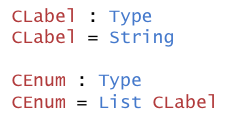
\includegraphics[scale=0.5]{Figures/AnInformativeEncodingofConstructorsLabels.png}
}
\subcaptionbox{Example: Constructors of Vec\label{fig:vectctors}}[.45\textwidth]{
    
\includegraphics[scale=0.5]{Figures/VectorConstructors.png}

}
\caption{Constructor Labels}
\end{center}
\end{figure}

Now that it is possible to represent the available constructors, we can encode a way of choosing a particular constructor tag. Figure~\ref{fig:ctortags} shows a datatype \tttype{Tag} with two constructors:
\ttconstructor{TZ} which represents the constructor that is on top of the current list and \ttconstructor{TS} which represents a constructor further along the list. As such, \tttype{Tag} specifies a valid index into a (non-empty) list of constructor tags.

This encoding has multiple advantages: it ensures that all constructor labels stored in our data exist in the expected list of constructors, it ensures that all datatypes which are dependent on a tag must have at least one constructor, and as a consequence
it is possible to specify the empty type by simply requiring a tag on an empty list of expected constructors (since such value would be impossible to create).
This encoding eases the implementation of automatically retrieving a tag given a constructor label using tactics in Idris, which might save some time when values
are constructed manually.

\begin{figure}[ht]
\begin{center}
    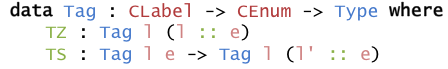
\includegraphics[scale=0.5]{Figures/AnInformativeEncodingofConstructorsTags.png}
\end{center}
\caption{Tags: A Structure for Picking a Constructor from a Label Collection}
\label{fig:ctortags}
\end{figure}

For the constructors of \tttype{Vec}, Figure~\ref{fig:vecctor} shows an example on what the tag values are. For \ttconstructor{Nil} the value is \ttconstructor{TZ} since it is the first in the list of \ttdec{VecCtors}, and for \ttconstructor{Cons} the value
is \ttconstructor{TS~TZ} since it is the second. Since there are only two elements in \ttdec{VecCtors}, it shouldn't be possible to create any other valid constructor tag, and as such it is a good representative for enumerating the constructors of \tttype{Vec}.

\begin{figure}[ht]
\begin{center}
  \subcaptionbox{Tag for \ttconstructor{Nil}\label{fig:vecctornil}}[.45\textwidth]{
    
\includegraphics[scale=0.5]{Figures/VectorNilTag.png}
}
\subcaptionbox{Tag for \ttconstructor{Cons}\label{fig:vecctorcons}}[.45\textwidth]{
    
\includegraphics[scale=0.5]{Figures/VectorConsTag.png}

}
\caption{Example: Tags for constructors of \tttype{Vec}}
\label{fig:vecctor}
\end{center}
\end{figure}


\subsection{A constructive type of choice}
\label{sub:AConstructiveTypeofChoice}
Similarly to how \texttt{\textbf{if}} was used to map \tttype{Bool} values to the descriptions of the various constructors of a datatype in Section~\ref{sub:ADescriptionforDatatypes}, it is desirable to have a way
to map \tttype{Tag} values.  The following section will describe the \ttdec{switch} function that allows mapping \tttype{Tag} values to suitable values of a desired type.

Since the number of constructors for a datatype can vary in length, it is necessary to calculate a type that allows mapping the tag of each constructor to a suitable value (shown in Figure~\ref{fig:smallpiop}). 
It is essentially a function that provides a one-to-one mapping from the list of constructors to a series of right-nested pairs ending with \tttype{()}.
The type of the resulting value \ttvar{prop} can be dependent on the input constructor tag, and therefore the function is called $\pi$ or the \textit{small pi operator}.
The operator $\pi$ is small in the sense that unlike the dependent function type $\Pi$ which allows the result to dependent on any type of input, $\pi$ only allows dependencies on constructor tags.

\begin{figure}[ht]
\begin{center}
    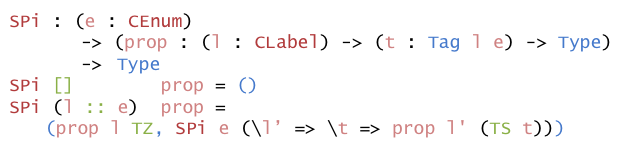
\includegraphics[scale=0.5]{Figures/AConstructiveTypeofChoice.png}
\end{center}
\caption{The Small Pi Operator: Type for Case Analysis based on Constructor Tags}
\label{fig:smallpiop}
\end{figure}

Given a way to map a list of constructors to a list of values using $\pi$, it is now possible to define \ttdec{switch} which can look up the corresponding result value in the map for a particular \tttype{Tag}.
The function \ttdec{switch} is shown in Figure~\ref{fig:switchctor} and has two branches: if the constructor to map is the first one in a list of constructors, it simply returns the first value in the corresponding mapping, otherwise
it continues the search using the rest of the provided elements (skipping the first constructor and its corresponding mapping).
Since there can be no value of \tttype{Tag} on an empty enumeration of constructors, it is not required to handle such case as the elaborator would automatically find out that such case is impossible.

\begin{figure}[ht]
\begin{center}
    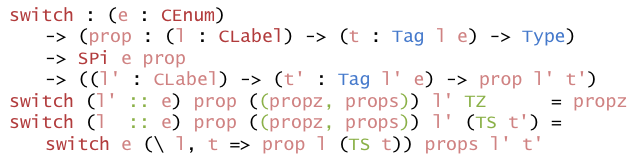
\includegraphics[scale=0.5]{Figures/AConstructiveChoice.png}
\end{center}
\caption{Calculation of a Property based on a Specific Constructor Tag}
\label{fig:switchctor}
\end{figure}

As an example, Figure~\ref{fig:vecdescim} shows the description of \tttype{Vec} (from Figure~\ref{fig:descvec}) again, but this time using the new constructor tag encoding instead of a Boolean variable.
While the description might initially seem more complicated than before, it has a couple of clear advantages: the encoding now contain the constructor tag and it is possible to choose between more than two constructors at the same time.

\begin{figure}[H]
\begin{center}
    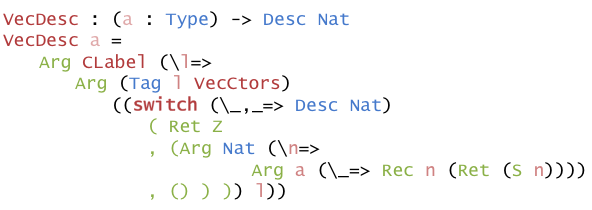
\includegraphics[scale=0.5]{Figures/VectorDescriptionImproved.png}
\end{center}
\caption{Description of Vec given a Constructor Tag}
\label{fig:vecdescim}
\end{figure}

\section{Synthesising descriptions to types}
\label{sec:SynthesisingDescriptionstoTypes}
In Section~\ref{sec:TheGenericStructureofInductiveDataTypes} I had shown how it was possible to create descriptions that support many common datatypes in Idris.
In this section I will present a way to convert or \textit{synthesise} these descriptions to actual types, that allows the programmer to construct values of these described types with actual data.

\subsection{A heterogeneous form of equality}
\label{sub:AHeterogeneousFormofEquality}
Before we proceed with the actual synthesis I would like to present one of the important types that is needed.
The type is called heterogeneous equality and is built into the core language theory of Idris.
\begin{figure}[ht]
\begin{center}
    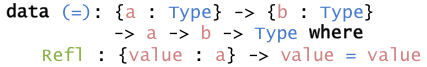
\includegraphics[scale=0.5]{Figures/HeterogeneousEquality.png}
\end{center}
\caption{Heterogeneous Equality of Values}
\label{fig:heteq}
\end{figure}
Heterogeneous equality takes two values of different types and constructors a type.
In order to actually construct a value of such type (i.e., provide a proof for the equality), we have to use \ttconstructor{Refl} which will only succeed if the compiler believes that such two values (and their types) are really the same.
This provides a simple yet powerful way to constrain values in order to ensure that any given input must conform to some expected form.

\subsection{Datatype synthesis}
\label{sub:DatatypeSynthesis}
It is finally time to convert the description to an actual type. Figure~\ref{fig:synthdata} shows the \ttdec{Synthesise} method which takes a description, the final form of that datatype and the resulting index, then it returns a type which can contain the described data.

\begin{itemize}
  \item If we reach the end of the description \textit{i.e.}, \ttconstructor{Ret}, the only thing that we need to ensure is that the provided resulting index matches the expected index provided in the description. In order to apply such constraint we use the heterogeneous equality type (see Section~\ref{sub:AHeterogeneousFormofEquality}).
  \item For recursive arguments \textit{i.e.}, \ttconstructor{Rec}, we construct a dependent pair where the first argument contains a value of the fully-synthesised type with the given index and the second argument contains the synthesised version of the rest of the provided description. The reason that we need the final form of the datatype in order to construct a recursive argument is due to the fact that if we call \ttdec{Synthesise} recursively on that argument we would get stuck in an infinite loop!
  \item For ordinary arguments \textit{i.e.}, \ttconstructor{Arg}, we also create a dependent pair. The first argument of the dependent pair is a value \ttvar{arg} of the provided type \ttvar{a}, and the second argument is the synthesis of the rest of the provided description \ttvar{d} given \ttvar{arg}. This is isomorphic to how an ordinary constructor would store the data and as such the dependent pair serves a good target structure for our synthesis.
\end{itemize}
Since the dependent pair is used as the target type for the synthesis, it itself must be a core part of the type theory similarly to the heterogeneous equality, if we want to treat all datatype declarations as describable.

\begin{figure}[ht]
\begin{center}
    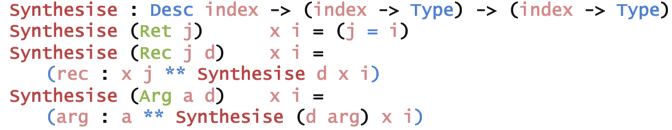
\includegraphics[scale=0.5]{Figures/SynthesisingData.png}
\end{center}
\caption{Synthesising Descriptions into Actual Types}
\label{fig:synthdata}
\end{figure}

We are able to synthesise our descriptions to actual types using \ttdec{Synthesise}; However, an issue occurs when we want to use it since it requires the final form of the described datatype as input but the only way to synthesise the datatype is using \ttdec{Synthesise} itself.
In order to ``tie the knot'' and complete input for \ttdec{Synthesise}, we define a final datatype \tttype{Data} that takes a description and provides the final form of the described datatype (see Figure~\ref{fig:datafromdesc}).
\tttype{Data} has only one constructor namely \ttconstructor{Con} which takes as input the synthesised version of the description \ttvar{d} with \tttype{Data}~\ttvar{d} serving as argument for the final form of the datatype in \ttdec{Synthesise}. This works since each time we face a recursive argument it must be constructed using \ttconstructor{Con} which avoids a infinite loop in \ttdec{Synthesise} as long as the elements that are constructed are smaller in size; Luckily, the typesystem of Idris ensures \textit{totality} of functions and as such doesn't permit the creation of values that are infinitely sized except when the arguments are explicitly declared as such using the \tttype{Inf} type.

\begin{figure}[ht]
\begin{center}
    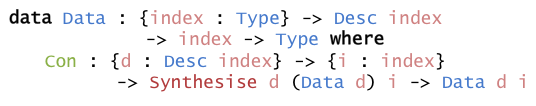
\includegraphics[scale=0.5]{Figures/TyingTheSynthesisKnot.png}
\end{center}
\caption{Knot-tying the Synthesised Description with Itself}
\label{fig:datafromdesc}
\end{figure}

\subsection{Example: Constructing vectors}
\label{sub:Example:Constructing Vectors}

To get a more concrete intuition on how it is possible to construct data values of described types, this section will look at the synthesised version of \tttype{Vec}.
Figure~\ref{fig:synthversvecdesc} shows \ttdec{Vec} which is a function mimicking its corresponding type constructor, and it even shares the same type signature.
The function \ttdec{Vec} returns a described type using \tttype{Desc} passing along the description of \tttype{Vec} and its required parameters (\textit{i.e.}, \ttdec{VecDesc}~\ttvar{a}), 
and additionally the expected value of the result index (\textit{i.e.}, \ttvar{n}).

\begin{figure}[ht]
\begin{center}
    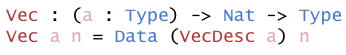
\includegraphics[scale=0.5]{Figures/VectorSynthesisedDesc.png}
\end{center}
\caption{Synthesised Version of Vector Description}
\label{fig:synthversvecdesc}
\end{figure}

A simple example representing the vector \ttconstructor{[}\ttliteral{1}~\ttconstructor{,}~\ttliteral{2}~\ttconstructor{,}~\ttliteral{3}\ttconstructor{]} is presented in Figure~\ref{fig:exmvecsynthvecdesc}. Although the value might seem a bit overwhelming at first, it follows a simple pattern:
Each time a value of \ttdec{Vec} is needed \ttconstructor{Con} is used, then it is followed by its required arguments in the form of nested dependent pairs, and finally it ends with \ttconstructor{Refl} which ensures
that the provided index of the value match up with the expected one.
As such, it can be observed that there are 4 occurences of \ttconstructor{Con} and \ttconstructor{Refl} in the example, three for the various applications
of \ttconstructor{Cons} and one for the application of \ttconstructor{Nil}. For all cases the first two arguments represent the constructor label and associated tag. 
For \ttconstructor{Cons} the first following argument is the length of the rest of the vector (the value of index \ttvar{n}) followed by the value of the list head and the list tail, ending with \ttconstructor{Refl}.
For \ttconstructor{Nil} the value is ended with \ttconstructor{Refl} since it doesn't contain any data.


\begin{figure}[ht]
\begin{center}
    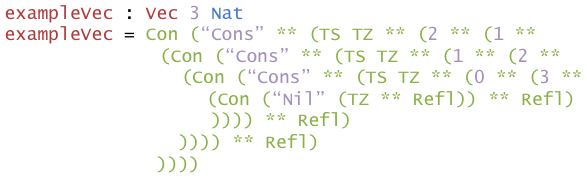
\includegraphics[scale=0.5]{Figures/VectorSynthesisedExample.png}
\end{center}
\caption{Example Vector representing \ttconstructor{[}\ttliteral{1}~\ttconstructor{,}~\ttliteral{2}~\ttconstructor{,}~\ttliteral{3}\ttconstructor{]} as a Value of a Synthesised Description}
\label{fig:exmvecsynthvecdesc}
\end{figure}

As might have become apparent there are a couple of shortcomings in the example, or rather the way values of described types are constructed.
One shortcoming is that there is a lot of boilerplate required when values are constructed, which makes the result somewhat unreadable.
A solution to overcome that shortcoming is presented in the next paragraph. Another shortcoming is that the resulting terms seem to become very large (and in turn slows down program execution) compared to the original
version of the datatype. For example, \ttconstructor{Nil} becomes inflated to \ttconstructor{Con~(}\ttliteral{"Nil"}~\ttconstructor{** (TZ ** Refl))} which is significantly more complex. A description on how to improve the size of resulting terms and
speed up the performance of dependent programs is presented in Chapter~\ref{cha:OptimizingIdrisforFlight}.

In order to make creation of values of described types easier and the resulting terms more readable, it is possible to use functions as synonyms for the constructors.
Figure~\ref{fig:funcconstrsynthvec} shows \ttdec{Nil} and \ttdec{Cons} as synonyms for the described version of \ttconstructor{Nil} and \ttconstructor{Cons} respectively.

\begin{figure}[ht]
\begin{center}
    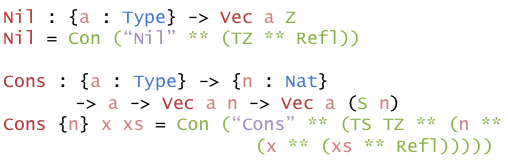
\includegraphics[scale=0.5]{Figures/VectorSynthesisedConstructors.png}
\end{center}
\caption{Functions for Constructing Values of Synthesised Vector Description}
\label{fig:funcconstrsynthvec}
\end{figure}

Using the provided synonyms, the constructor of the value in example in Figure~\ref{fig:exmvecsynthvecdesc} becomes simpler and much more readable. Figure~\ref{fig:exmvecsynthvecdescconstrs} shows the updated version,
and it looks almost exactly like the original value it needed to describe \ttliteral{[1, 2, 3]}.


\begin{figure}[ht]
\begin{center}
    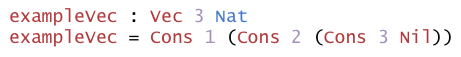
\includegraphics[scale=0.5]{Figures/VectorSynthesisedConstructorsExample.png}
\end{center}
\caption{More Readable Version of \ttconstructor{[}\ttliteral{1}~\ttconstructor{,}~\ttliteral{2}~\ttconstructor{,}~\ttliteral{3}\ttconstructor{]}  using previously-defined Aliases}
\label{fig:exmvecsynthvecdescconstrs}
\end{figure}

\section{The (mostly) gentle art of levitation}
\label{sec:TheMostlyGentleArtofLevitation}
In the previous sections, I had presented a series of constructions that makes it possible to have described types.
What may have become apparent for the user is that many of these constructions such as \tttype{Data}, \tttype{Tag} and \ttdec{switch} cannot themselves be described since
they are necessary dependencies for having descriptions.
However, what might be surprising is that the description type itself \tttype{Desc}, isn't in fact limited by such constraint
and can be described itself.
This is the key point addressed by \cite{Chapman:2010:GAL:1863543.1863547} in "The gentle art of levitation".

The description datatype \tttype{Desc} contains many of the constructors needed to describe itself.
However, one might experience trouble when trying to describe \ttconstructor{Arg} since it requires an argument of the following type:
\texttt{(}\ttvar{a}~->\tttype{Desc}~\ttvar{ix}\texttt{)}.
This argument describes a function which result type is the datatype itself (a so-called higher-order inductive argument), which \ttconstructor{Rec} isn't strong enough to express since it only permits recursive values.
Figure~\ref{fig:deschrec} shows a new constructor \ttconstructor{HRec}, which allows specification of such higher-order inductive arguments taking a type \ttvar{a} which specifies
the expected input type of such argument in addition to the rest of arguments that are expected by \ttconstructor{Rec}.

\begin{figure}[ht]
\begin{center}
    
\includegraphics[scale=0.5]{Figures/ADescriptionForDatatypesExtended.png}
\end{center}
\caption{A constructor for \tttype{Desc} to represent higher-order recursion}
\label{fig:deschrec}
\end{figure}

Similarly to the other constructors of \tttype{Desc}, \ttdec{Synthesise} must be extended with a clause for \ttconstructor{HRec}. Figure~\ref{fig:synthhrec} shows the corresponding clause,
which looks very similar to the one for \ttconstructor{Rec}, except the first component now requires a function from the provided type \ttvar{a} to the datatype itself instead of just a reference
to the datatype.

\begin{figure}[ht]
\begin{center}
    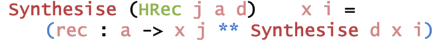
\includegraphics[scale=0.5]{Figures/SynthesisingDataExtended.png}
\end{center}
\caption{Synthesising \ttconstructor{HRec} to a real type}
\label{fig:synthhrec}
\end{figure}

Finally, all the required constructors are present and it is now possible to piece together a description for \tttype{Desc}. Figure~\ref{fig:descdesc} shows the complete description, including for the newly added
\ttconstructor{HRec} constructor. The description of \tttype{Desc} is parametrised by the type of indices \ttvar{ix} that possible derived descriptions can have, and is not indexed by anything particularly interesting (the unit type \tttype{()} is used in the figure).
For each constructor, it matches the original definition presented Figure~\ref{fig:descriptiondatatype}. The only interesting case is the one for \ttconstructor{Arg}, which uses \ttconstructor{HRec ()}~\ttvar{a}~\texttt{(}\ttconstructor{Ret ()}\texttt{)} to represent the higher-order inductive argument \texttt{(}\ttvar{a}~->~\tttype{Desc}~\ttvar{ix}\texttt{)}.

\begin{figure}[ht]
\begin{center}
    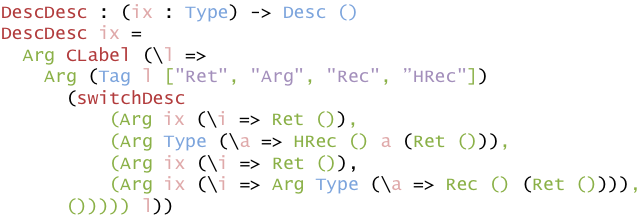
\includegraphics[scale=0.5]{Figures/DescriptionDescription.png}
\end{center}
\caption{Describing the \tttype{Desc} datatype itself}
\label{fig:descdesc}
\end{figure}

Perhaps, the key thing to notice is that a function \ttdec{switchDesc} was used instead of \ttdec{switch} when describing \tttype{Desc}.
Figure~\ref{fig:switchdesc} shows how \ttdec{switchDesc} is defined by specialising \ttdec{switch}. However, if \tttype{Desc} is a described type based on \ttdec{DescDesc} then such definition would be circular.
This is because the general \ttdec{switch} requires the result type \tttype{Desc} to be given as argument, but \tttype{Desc} is dependent on \ttdec{DescDesc}. Therefore, \cite{Chapman:2010:GAL:1863543.1863547} define \ttdec{switchDesc} to be handled specially in their type theory, eliding the definition of the body
and hard-wiring its return type to be \tttype{Desc}\footnote{Of course, such trick only works if there is know to be a type \tttype{Desc} in the meta-theory. However, the knowledge of its elements is not necessarily required and it is possible to inspect these
in a similar fashion to other datatypes.}. Now, \ttdec{DescDesc} can be type checked without any issues and \textit{levitation} is achieved.

\begin{figure}[ht]
\begin{center}
    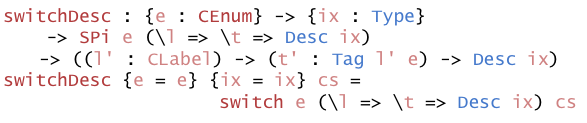
\includegraphics[scale=0.5]{Figures/AConstructiveChoiceDesc.png}
\end{center}
\caption{A specialised version of \ttdec{switch} which returns descriptions}
\label{fig:switchdesc}
\end{figure}

\chapter{Partial evaluation}
\label{cha:PartialEvaluation}

\section{Functions and constant inputs}
\label{sec:FunctionsandConstantInputs}
\textit{General introduction about partial evaluation.}

\section{Binding-time analyses of programs}
\label{sec:Binding-timeAnalysisofPrograms}
\textit{Finding the relevant constant parts of the program.}

\section{Specialisation as a form of optimisation}
\label{sec:SpecialisationasaFormofOptimization}
\textit{Performance benefits of program specialisation. Pitfalls.}

\chapter{Levitating Idris}
\label{cha:LevitatingIdris}

\section{A pragmatic implementation of levitation}
\label{sec:APragmaticImplementationofLevitation}
\textit{How the general concept of levitation was transferred to Idris.}

\section{Description synthesis from ordinary data declarations}
\label{sec:DescriptionSynthesisFromOrdinaryDataDeclarations}
\textit{How ordinary data-declarations are synthesized to levitational descriptions.}

\chapter{Practical examples}
\label{cha:PracticalExamples}

\section{Generic deriving}
\label{sec:GenericDeriving}
\textit{Examples of generic deriving of algorithms like decidable equality, pretty printing and possibly eliminators via generic structure.}

\section{Uniplate for Idris}
\label{sec:UniplateforIdris}
\textit{A version of the Uniplate library for Idris based on} \url{http://community.haskell.org/~ndm/uniplate/} \textit{and} \url{http://www-ps.informatik.uni-kiel.de/~sebf/projects/traversal.html} \textit{.
This is useful for traversing structures in a generic fashion and especially when dealing with small changes in large data structures (such as compiler ADTs)}

\chapter{Optimising Idris for flight}
\label{cha:OptimizingIdrisforFlight}

\section{Specialising constructors for specific types}
\label{sec:SpecialisingConstructorsforSpecificTypes}
\textit{How generalized constructors of described types, are specialised as ordinary data structures.}

\section{Online erasure of unused arguments}
\label{sec:OnlineErasureofUnusedArguments}
\textit{How some type infromation is to be erased at compile time to reduce elaboration overhead. Very hypothetical.}

\section{Static initialization of generic functions}
\label{sec:StaticInitializationofGenericFunctions}
\textit{How algorithms that are dependent on the generic structure of a datatype are optimised. Discuss benefits of having a JIT/Profiling information for future work.}

\chapter{Evaluation}
\label{cha:Evaluation}

\chapter{Discussion}
\label{cha:Discussion}

\section{Future work}
\label{sec:FutureWork}

\section{Conclusion}
\label{sec:Conclusion}

\appendix
\bibliography{report.bib}
\end{document}
